% Options for packages loaded elsewhere
% Options for packages loaded elsewhere
\PassOptionsToPackage{unicode}{hyperref}
\PassOptionsToPackage{hyphens}{url}
\PassOptionsToPackage{dvipsnames,svgnames,x11names}{xcolor}
%
\documentclass[
  letterpaper,
  DIV=11,
  numbers=noendperiod]{scrartcl}
\usepackage{xcolor}
\usepackage{amsmath,amssymb}
\setcounter{secnumdepth}{-\maxdimen} % remove section numbering
\usepackage{iftex}
\ifPDFTeX
  \usepackage[T1]{fontenc}
  \usepackage[utf8]{inputenc}
  \usepackage{textcomp} % provide euro and other symbols
\else % if luatex or xetex
  \usepackage{unicode-math} % this also loads fontspec
  \defaultfontfeatures{Scale=MatchLowercase}
  \defaultfontfeatures[\rmfamily]{Ligatures=TeX,Scale=1}
\fi
\usepackage{lmodern}
\ifPDFTeX\else
  % xetex/luatex font selection
\fi
% Use upquote if available, for straight quotes in verbatim environments
\IfFileExists{upquote.sty}{\usepackage{upquote}}{}
\IfFileExists{microtype.sty}{% use microtype if available
  \usepackage[]{microtype}
  \UseMicrotypeSet[protrusion]{basicmath} % disable protrusion for tt fonts
}{}
\makeatletter
\@ifundefined{KOMAClassName}{% if non-KOMA class
  \IfFileExists{parskip.sty}{%
    \usepackage{parskip}
  }{% else
    \setlength{\parindent}{0pt}
    \setlength{\parskip}{6pt plus 2pt minus 1pt}}
}{% if KOMA class
  \KOMAoptions{parskip=half}}
\makeatother
% Make \paragraph and \subparagraph free-standing
\makeatletter
\ifx\paragraph\undefined\else
  \let\oldparagraph\paragraph
  \renewcommand{\paragraph}{
    \@ifstar
      \xxxParagraphStar
      \xxxParagraphNoStar
  }
  \newcommand{\xxxParagraphStar}[1]{\oldparagraph*{#1}\mbox{}}
  \newcommand{\xxxParagraphNoStar}[1]{\oldparagraph{#1}\mbox{}}
\fi
\ifx\subparagraph\undefined\else
  \let\oldsubparagraph\subparagraph
  \renewcommand{\subparagraph}{
    \@ifstar
      \xxxSubParagraphStar
      \xxxSubParagraphNoStar
  }
  \newcommand{\xxxSubParagraphStar}[1]{\oldsubparagraph*{#1}\mbox{}}
  \newcommand{\xxxSubParagraphNoStar}[1]{\oldsubparagraph{#1}\mbox{}}
\fi
\makeatother

\usepackage{color}
\usepackage{fancyvrb}
\newcommand{\VerbBar}{|}
\newcommand{\VERB}{\Verb[commandchars=\\\{\}]}
\DefineVerbatimEnvironment{Highlighting}{Verbatim}{commandchars=\\\{\}}
% Add ',fontsize=\small' for more characters per line
\usepackage{framed}
\definecolor{shadecolor}{RGB}{241,243,245}
\newenvironment{Shaded}{\begin{snugshade}}{\end{snugshade}}
\newcommand{\AlertTok}[1]{\textcolor[rgb]{0.68,0.00,0.00}{#1}}
\newcommand{\AnnotationTok}[1]{\textcolor[rgb]{0.37,0.37,0.37}{#1}}
\newcommand{\AttributeTok}[1]{\textcolor[rgb]{0.40,0.45,0.13}{#1}}
\newcommand{\BaseNTok}[1]{\textcolor[rgb]{0.68,0.00,0.00}{#1}}
\newcommand{\BuiltInTok}[1]{\textcolor[rgb]{0.00,0.23,0.31}{#1}}
\newcommand{\CharTok}[1]{\textcolor[rgb]{0.13,0.47,0.30}{#1}}
\newcommand{\CommentTok}[1]{\textcolor[rgb]{0.37,0.37,0.37}{#1}}
\newcommand{\CommentVarTok}[1]{\textcolor[rgb]{0.37,0.37,0.37}{\textit{#1}}}
\newcommand{\ConstantTok}[1]{\textcolor[rgb]{0.56,0.35,0.01}{#1}}
\newcommand{\ControlFlowTok}[1]{\textcolor[rgb]{0.00,0.23,0.31}{\textbf{#1}}}
\newcommand{\DataTypeTok}[1]{\textcolor[rgb]{0.68,0.00,0.00}{#1}}
\newcommand{\DecValTok}[1]{\textcolor[rgb]{0.68,0.00,0.00}{#1}}
\newcommand{\DocumentationTok}[1]{\textcolor[rgb]{0.37,0.37,0.37}{\textit{#1}}}
\newcommand{\ErrorTok}[1]{\textcolor[rgb]{0.68,0.00,0.00}{#1}}
\newcommand{\ExtensionTok}[1]{\textcolor[rgb]{0.00,0.23,0.31}{#1}}
\newcommand{\FloatTok}[1]{\textcolor[rgb]{0.68,0.00,0.00}{#1}}
\newcommand{\FunctionTok}[1]{\textcolor[rgb]{0.28,0.35,0.67}{#1}}
\newcommand{\ImportTok}[1]{\textcolor[rgb]{0.00,0.46,0.62}{#1}}
\newcommand{\InformationTok}[1]{\textcolor[rgb]{0.37,0.37,0.37}{#1}}
\newcommand{\KeywordTok}[1]{\textcolor[rgb]{0.00,0.23,0.31}{\textbf{#1}}}
\newcommand{\NormalTok}[1]{\textcolor[rgb]{0.00,0.23,0.31}{#1}}
\newcommand{\OperatorTok}[1]{\textcolor[rgb]{0.37,0.37,0.37}{#1}}
\newcommand{\OtherTok}[1]{\textcolor[rgb]{0.00,0.23,0.31}{#1}}
\newcommand{\PreprocessorTok}[1]{\textcolor[rgb]{0.68,0.00,0.00}{#1}}
\newcommand{\RegionMarkerTok}[1]{\textcolor[rgb]{0.00,0.23,0.31}{#1}}
\newcommand{\SpecialCharTok}[1]{\textcolor[rgb]{0.37,0.37,0.37}{#1}}
\newcommand{\SpecialStringTok}[1]{\textcolor[rgb]{0.13,0.47,0.30}{#1}}
\newcommand{\StringTok}[1]{\textcolor[rgb]{0.13,0.47,0.30}{#1}}
\newcommand{\VariableTok}[1]{\textcolor[rgb]{0.07,0.07,0.07}{#1}}
\newcommand{\VerbatimStringTok}[1]{\textcolor[rgb]{0.13,0.47,0.30}{#1}}
\newcommand{\WarningTok}[1]{\textcolor[rgb]{0.37,0.37,0.37}{\textit{#1}}}

\usepackage{longtable,booktabs,array}
\usepackage{calc} % for calculating minipage widths
% Correct order of tables after \paragraph or \subparagraph
\usepackage{etoolbox}
\makeatletter
\patchcmd\longtable{\par}{\if@noskipsec\mbox{}\fi\par}{}{}
\makeatother
% Allow footnotes in longtable head/foot
\IfFileExists{footnotehyper.sty}{\usepackage{footnotehyper}}{\usepackage{footnote}}
\makesavenoteenv{longtable}
\usepackage{graphicx}
\makeatletter
\newsavebox\pandoc@box
\newcommand*\pandocbounded[1]{% scales image to fit in text height/width
  \sbox\pandoc@box{#1}%
  \Gscale@div\@tempa{\textheight}{\dimexpr\ht\pandoc@box+\dp\pandoc@box\relax}%
  \Gscale@div\@tempb{\linewidth}{\wd\pandoc@box}%
  \ifdim\@tempb\p@<\@tempa\p@\let\@tempa\@tempb\fi% select the smaller of both
  \ifdim\@tempa\p@<\p@\scalebox{\@tempa}{\usebox\pandoc@box}%
  \else\usebox{\pandoc@box}%
  \fi%
}
% Set default figure placement to htbp
\def\fps@figure{htbp}
\makeatother


% definitions for citeproc citations
\NewDocumentCommand\citeproctext{}{}
\NewDocumentCommand\citeproc{mm}{%
  \begingroup\def\citeproctext{#2}\cite{#1}\endgroup}
\makeatletter
 % allow citations to break across lines
 \let\@cite@ofmt\@firstofone
 % avoid brackets around text for \cite:
 \def\@biblabel#1{}
 \def\@cite#1#2{{#1\if@tempswa , #2\fi}}
\makeatother
\newlength{\cslhangindent}
\setlength{\cslhangindent}{1.5em}
\newlength{\csllabelwidth}
\setlength{\csllabelwidth}{3em}
\newenvironment{CSLReferences}[2] % #1 hanging-indent, #2 entry-spacing
 {\begin{list}{}{%
  \setlength{\itemindent}{0pt}
  \setlength{\leftmargin}{0pt}
  \setlength{\parsep}{0pt}
  % turn on hanging indent if param 1 is 1
  \ifodd #1
   \setlength{\leftmargin}{\cslhangindent}
   \setlength{\itemindent}{-1\cslhangindent}
  \fi
  % set entry spacing
  \setlength{\itemsep}{#2\baselineskip}}}
 {\end{list}}
\usepackage{calc}
\newcommand{\CSLBlock}[1]{\hfill\break\parbox[t]{\linewidth}{\strut\ignorespaces#1\strut}}
\newcommand{\CSLLeftMargin}[1]{\parbox[t]{\csllabelwidth}{\strut#1\strut}}
\newcommand{\CSLRightInline}[1]{\parbox[t]{\linewidth - \csllabelwidth}{\strut#1\strut}}
\newcommand{\CSLIndent}[1]{\hspace{\cslhangindent}#1}



\setlength{\emergencystretch}{3em} % prevent overfull lines

\providecommand{\tightlist}{%
  \setlength{\itemsep}{0pt}\setlength{\parskip}{0pt}}



 


\KOMAoption{captions}{tableheading}
\makeatletter
\@ifpackageloaded{caption}{}{\usepackage{caption}}
\AtBeginDocument{%
\ifdefined\contentsname
  \renewcommand*\contentsname{Table of contents}
\else
  \newcommand\contentsname{Table of contents}
\fi
\ifdefined\listfigurename
  \renewcommand*\listfigurename{List of Figures}
\else
  \newcommand\listfigurename{List of Figures}
\fi
\ifdefined\listtablename
  \renewcommand*\listtablename{List of Tables}
\else
  \newcommand\listtablename{List of Tables}
\fi
\ifdefined\figurename
  \renewcommand*\figurename{Figure}
\else
  \newcommand\figurename{Figure}
\fi
\ifdefined\tablename
  \renewcommand*\tablename{Table}
\else
  \newcommand\tablename{Table}
\fi
}
\@ifpackageloaded{float}{}{\usepackage{float}}
\floatstyle{ruled}
\@ifundefined{c@chapter}{\newfloat{codelisting}{h}{lop}}{\newfloat{codelisting}{h}{lop}[chapter]}
\floatname{codelisting}{Listing}
\newcommand*\listoflistings{\listof{codelisting}{List of Listings}}
\makeatother
\makeatletter
\makeatother
\makeatletter
\@ifpackageloaded{caption}{}{\usepackage{caption}}
\@ifpackageloaded{subcaption}{}{\usepackage{subcaption}}
\makeatother
\usepackage{bookmark}
\IfFileExists{xurl.sty}{\usepackage{xurl}}{} % add URL line breaks if available
\urlstyle{same}
\hypersetup{
  pdftitle={Gjennomrettet},
  pdfauthor={Ny gruppe 0001, kandidatnummer 170011 og 170029},
  colorlinks=true,
  linkcolor={blue},
  filecolor={Maroon},
  citecolor={Blue},
  urlcolor={Blue},
  pdfcreator={LaTeX via pandoc}}


\title{Gjennomrettet}
\usepackage{etoolbox}
\makeatletter
\providecommand{\subtitle}[1]{% add subtitle to \maketitle
  \apptocmd{\@title}{\par {\large #1 \par}}{}{}
}
\makeatother
\subtitle{Term paper in ECON 3170/4170, autumn 2026}
\author{Ny gruppe 0001, kandidatnummer 170011 og 170029}
\date{Invalid Date}
\begin{document}
\maketitle

\renewcommand*\contentsname{Table of contents}
{
\hypersetup{linkcolor=}
\setcounter{tocdepth}{3}
\tableofcontents
}

\subsection{Abstract}\label{abstract}

Denne oppgaven undersøker sammenhengen mellom Norgespris, strømpriser og
husholdningenes strømforbruk i Norge. Med utgangspunkt i data fra Nord
Pool, Elhub og NVE for perioden 2020--2026 analyseres forskjeller i
strømforbruk mellom husholdninger med ulik Norgespris-adopsjon,
sammenhengen mellom strømpriser og nye signeringer av Norgespris, samt
forholdet mellom magasinfylling og spotpriser. Analysen kombinerer
deskriptiv statistikk med OLS- og LASSO-regresjon for å undersøke
statistiske sammenhenger og modellens prediksjonsevne. Resultatene viser
en negativ sammenheng mellom magasinfylling og spotpriser, mens OLS og
LASSO har tilnærmet lik prediksjonsevne i analysen av husholdningenes
strømforbruk. Legg til resultat fra problemstilling 2.

\subsection{1. Introduksjon og objektiv}\label{introduksjon-og-objektiv}

Strømprisene i Norge har hatt betydelige svingninger de siste årene,
særlig mellom de ulike prisområdene. I 2021 nådde strømprisene
historiske nivåer, spesielt i Sør-Norge (NO1 og NO2). Dette ble blant
annet knyttet til høye kraftpriser i Europa og lavere magasinfylling enn
normalt (Skaansar 2022). Som følge av prisutviklingen innførte
regjeringen strømstøtte i desember 2021 (kontor, Energidepartementet,
and Finansdepartementet 2021).

Den 1. oktober 2025 innførte regjeringen Norgespris, en frivillig
fastprisordning for strøm og fjernvarme. Ordningen ga husholdninger
mulighet til å velge en fastpris på 40 øre/kWh ekskl. mva.
(Energidepartementet 2025). I oktober 2026 ble det besluttet at
ordningen videreføres i 2027, med en justert pris på 45 øre/kWh ekskl.
mva. (Energidepartementet 2026).

Formålet med oppgaven er å undersøke sammenhengen mellom Norgespris,
strømpriser og husholdningenes strømforbruk i Norge.

\textbf{Vi undersøker følgende problemstillinger:}

\begin{enumerate}
\def\labelenumi{\arabic{enumi}.}
\item
  Hvordan varierer strømforbruket mellom husholdninger med og uten
  Norgespris?
\item
  Hvordan henger utviklingen i strømprisene sammen med husholdningenes
  adopsjon av Norgespris?
\item
  I hvilken grad kan fyllingsgraden i norske vannmagasiner bidra til å
  forklare variasjoner i strømprisene?
\end{enumerate}

Analysen bygger på data fra Nord Pool, Elhub og Norges vassdrags- og
energidirektorat (NVE). Vi kombinerer deskriptiv statistikk og grafisk
fremstilling med statistiske analyser og regresjonsmodeller for å
undersøke utviklingstrekk og sammenhenger i datamaterialet.

\subsection{2. Databehandling og
implementering}\label{databehandling-og-implementering}

Hele databehandlingsprosessen og de empiriske analysene er gjennomført i
R med følgende sekundærdata:

\begin{enumerate}
\def\labelenumi{\arabic{enumi}.}
\item
  Elhub: Daglige data for aggregert strømforbruk (kWh), antall
  målepunkter og Norgespris-adopsjon, fordelt på prisområdene NO1--NO5
  og forbruksgruppene husholdning og fritidsbolig (Sannes and Elhub
  2026b, 2026a; Stokke Hammer-Dybvad and Elhub 2026).
\item
  Norges vassdrags- og energidirektorat (NVE): Ukentlige data for
  fyllingsgraden i norske vannmagasiner (energidirektorat 2026).
\item
  Nord Pool: Daglige aggregerte spotpriser for perioden 2020--2026 og
  timepriser for perioden 1. oktober 2025--30. september 2026 (Nordpool
  2026a, 2026b).
\end{enumerate}

Rådataene er hentet i CSV- og Excel-format, bearbeidet individuelt også
kombinert til et felles datagrunnlag for analysene.

\subsubsection{2.1 Nord Pool}\label{nord-pool}

Fra Nord Pool benytter vi daglige aggregerte spotpriser for de fem
norske prisområdene (NO1--NO5) i perioden 2020--29. september 2026. I
tillegg benyttes timebaserte spotpriser for perioden 1. oktober
2025--30. september 2026.

Prisdataene ble lastet ned i separate Excel-filer og importert til R ved
hjelp av \texttt{readxl}. Filene ble kombinert til samlede datasett.
Metadata og ``NA'' observasjoner fjernet. Datoene ble standardisert og
sortert kronologisk. Timeprisene ble tilsvarende kombinert.

Prisene i begge datasettene er opprinnelig oppgitt i NOK/MWh. Vi har
konvertert til NOK/kWh ved å dele på 1000. Dette gir sammenlignbare
måleenheter på tvers av data. I tillegg er måleenheten for strømstøtte
og norgespris definert som støtte i NOK/kWh, og det er dermed naturlig å
ha dataen på denne enheten.

For timeprisene ble daglige oppsummeringsverdier (minimum, maksimum og
gjennomsnitt) skilt fra de ordinære timeobservasjonene for å unngå at
ulike tidsoppløsninger blandes i analysene.

\subsubsection{2.2 Elhub -- Norgespris og
strømforbruk}\label{elhub-norgespris-og-struxf8mforbruk}

Dataene ble importert fra CSV-filer og omstrukturert fra bredt til langt
format for å aggregere undergruppene til samlevariabler for
husholdninger og fritidsboliger. På bakgrunn av disse ble det beregnet
andeler av målepunkter med Norgespris og andeler av strømforbruket som
dekkes av ordningen. \textbf{Se vedlegg xx for å se utdrag/hele koden.
Strukturen og oppsettet av funksjonen er lik for alle datasettene.
\textless- Bendik}

Det er viktig å merke seg at antall målepunkter ikke nødvendigvis
tilsvarer antall husholdninger, ettersom én husholdning kan disponere
flere målepunkter.

\subsubsection{2.3 Konstruksjon av reell sluttpris og strømstøtte Bendik
du må sjekke at dette er riktig siden jeg ikke har jobba med
koden}\label{konstruksjon-av-reell-sluttpris-og-struxf8mstuxf8tte-bendik-du-muxe5-sjekke-at-dette-er-riktig-siden-jeg-ikke-har-jobba-med-koden}

For å undersøke hvilke prissignaler husholdningene står overfor,
beregnes en estimert sluttpris etter strømstøtte. Spotprisen alene gir
ikke et fullstendig bilde av husholdningenes faktiske priskostnad,
ettersom staten har gitt strømstøtte siden desember 2021.

Sluttprisen beregnes ved å trekke beregnet strømstøtte fra spotprisen.
Beregningen tar hensyn til historiske endringer i støtteordningens
dekningsgrad og innslagsterskel. Fra desember 2021 var støttesatsen
først 55 \%, før den ble økt til 80 \% og senere 90 \%.
Innslagsterskelen ble gradvis justert fra 70 øre/kWh til 77 øre/kWh i
2026.

Videre konstrueres Norgespris som en referansepris på 40 øre/kWh ekskl.
mva. (50 øre inkl. mva.) fra 1. oktober 2025.

Utdrag av funksjon for støtteutregner få vise datawrangling og utregning
av ny data? \textbf{Se vedlegg xx for å se utdrag/hele koden. Strukturen
og oppsettet av funksjonen er lik for alle datasettene. \textless-
Bendik}

\subsubsection{2.4 NVE -- fyllingsgrad i
vannmagasiner}\label{nve-fyllingsgrad-i-vannmagasiner}

For å undersøke sammenhengen mellom magasinfylling og strømpriser
benyttes ukentlige data fra Norges vassdrags- og energidirektorat (NVE)
for perioden 2020--2026, fordelt på de fem norske prisområdene.
Fyllingsgraden gir informasjon om tilgjengelige vannkraftressurser og
kan påvirke kraftprodusentenes vannverdier og forventninger om fremtidig
krafttilgang.

Excel-filene ble importert og bearbeidet i R. Relevante kolonner ble
hentet ut, og datasettene ble omstrukturert og slått sammen ved hjelp av
årstall og ukenummer som felles variabler. Manglende observasjoner ble
fjernet. Dataene ble deretter organisert i langt format, der hver
observasjon representerer fyllingsgraden i ett prisområde for en bestemt
uke. Med R-pakken \texttt{ISOweek} ble årstall og ISO-ukenummer
konvertert til kalenderdatoer, med mandag som referansedag. Til slutt
ble datasettet sortert etter prisområde og dato, og variabelnavnene
standardisert.

\subsection{3. Metode}\label{metode}

Analysen benytter ordinær minste kvadraters metode (OLS) og regularisert
regresjon (LASSO) for å undersøke statistiske sammenhenger og
prediksjonsevne. OLS benyttes som hovedmetode for å estimere
sammenhenger mellom variablene, mens LASSO brukes som en supplerende
metode for variabelseleksjon og prediksjon i problemstilling 1 og 2. I
problemstilling 1 og 2 sammenlignes også prediksjonsevnen til OLS og
LASSO på felles testsett. Databehandling og modellering er gjennomført i
R, med Tidyverse og Tidymodels som sentrale rammeverk (Wickham and
Grolemund 2016; Kuhn and Silge 2023).

Valget av estimeringsmetoder bygger på skillet mellom økonomisk
parameterestimering og prediksjon (Athey and Imbens 2019; Hammersmark
2026).

\subsubsection{3.1 Empirisk tilnærming og
datastruktur}\label{empirisk-tilnuxe6rming-og-datastruktur}

Analysen benytter data med ulik tidsoppløsning, tilpasset de enkelte
problemstillingene. Datagrunnlaget omfatter daglige og ukentlige
observasjoner for de fem norske strømprisområdene. For å kontrollere for
regionale forskjeller og tidsvariasjoner inkluderes områdespesifikke og
tidsrelaterte kontrollvariabler i modellene.

Den generelle modellstrukturen kan uttrykkes som: y\_\{it\} = \beta*0 +*
\boldsymbol{\beta}'\mathbf{X}{it} + \alpha\_i + \delta*m +*
\varepsilon{it}

Her representerer y\_\{it\}\$ den avhengige variabelen, mens \(X_{it}\)
er forklaringsvariablene. Områdespesifikke effekter \((\alpha_i)\)
fanger opp forskjeller mellom prisområdene. Tidsrelaterte
kontrollvariabler \((\delta_t)\) benyttes for å kontrollere for
sesongvariasjoner eller generelle tidstrender, avhengig av
problemstillingen.

\subsubsection{3.2 Estimerings- og
prediksjonsmetoder}\label{estimerings--og-prediksjonsmetoder}

\paragraph{3.2.1 Ordinær minste kvadraters metode
(OLS)}\label{ordinuxe6r-minste-kvadraters-metode-ols}

OLS benyttes til å estimere lineære sammenhenger mellom avhengige
variabler og forklaringsvariabler. Metoden estimerer koeffisientene ved
å minimere summen av kvadrerte residualer.

OLS benyttes i alle tre problemstillingene. I problemstilling 1 og 3
brukes metoden til å undersøke statistiske sammenhenger, mens den i
problemstilling 2 også benyttes som sammenligningsgrunnlag for
prediksjon.

\paragraph{3.2.2 Regularisert regresjon
(LASSO)}\label{regularisert-regresjon-lasso}

LASSO-regresjon (Least Absolute Shrinkage and Selection Operator)
benyttes som en supplerende metode i problemstilling 1 og 2. Metoden
kombinerer lineær regresjon med en (L\_1)-straff som begrenser
størrelsen på koeffisientene og kan sette mindre relevante koeffisienter
lik null. Dette muliggjør variabelseleksjon og kan redusere risikoen for
overtilpasning (Tibshirani 1996; Hastie, Tibshirani, and Friedman 2009;
Fonti 2017; Gentzkow, Kelly, and Taddy 2019).

LASSO-modellen estimeres ved å minimere:

\[
\hat{\boldsymbol{\beta}}_{\text{lasso}}
=
\arg\min_{\boldsymbol{\beta}}
\left[
\sum_{i=1}^{N}
\left(
y_i-\beta_0-\sum_{j=1}^{p}x_{ij}\beta_j
\right)^2
+
\lambda\sum_{j=1}^{p}|\beta_j|
\right]
\]

Straffeparameteren \((\lambda)\) bestemmer graden av regularisering. En
høyere verdi gir sterkere krymping av koeffisientene, mens en lavere
verdi gjør modellen mer lik ordinær lineær regresjon.

For å evaluere prediksjonsevnen deles datamaterialet i et treningssett
(80 \%) og et testsett (20 \%). Straffeparameteren velges gjennom
10-fold kryssvalidering på treningsdataene, med RMSE som utgangspunkt
for modellvalget. RMSE og (R\^{}2) benyttes i kryssvalideringen, mens
RMSE, (R\^{}2) og MAE benyttes ved evaluering på testsettet.
Prediksjonsevnen til OLS og LASSO sammenlignes på det samme testsettet.

\subsubsection{3.3 Modellspesifikasjoner}\label{modellspesifikasjoner}

De tre problemstillingene undersøker ulike sammenhenger i datasettet.
Modellene tilpasses derfor den enkelte problemstillingen med hensyn til
avhengig variabel, forklaringsvariabler og tidsrelaterte
kontrollvariabler.

\subsubsection{3.3.1 Norgespris og strømforbruk: Problemstilling
1}\label{norgespris-og-struxf8mforbruk-problemstilling-1}

Problemstillingen undersøker sammenhengen mellom andelen husholdningenes
strømforbruk som er knyttet til Norgespris og husholdningenes samlede
strømforbruk. Modellen inkluderer områdefaste effekter og månedseffekter
for å kontrollere for geografiske forskjeller og sesongvariasjoner.

For å undersøke sammenhengen spesifiseres følgende modell: \[
\text{forbruk\_hus}_{it}
= \beta_0
+ \beta_1 \text{prosent\_forbruk\_hus\_np}_{it}
+ \beta_2 \text{slutt\_average}_{it}
+ \alpha_i
+ \delta_m
+ \varepsilon_{it}
\]

Her er \(\text{forbruk\_hus}_{it}\) husholdningenes samlede strømforbruk
i prisområde \(i\) på tidspunkt \(t\), målt i kWh, mens
\(\text{prosent\_forbruk\_hus\_np}_{it}\) angir andelen av
husholdningenes samlede strømforbruk som er knyttet til Norgespris.
\(\text{slutt\_average}_{it}\) angir gjennomsnittlig strømpris etter
strømstøtte (NOK/kWh). \(\alpha_i\) representerer områdefaste effekter,
mens \(\delta_m\) representerer månedseffekter.

\begin{Shaded}
\begin{Highlighting}[]
\CommentTok{\# Estimering av OLS{-}modell med faste effekter for område og måned}
\NormalTok{modell\_p1 }\OtherTok{\textless{}{-}} \FunctionTok{lm}\NormalTok{(}
\NormalTok{  forbruk\_hus }\SpecialCharTok{\textasciitilde{}}\NormalTok{ prosent\_forbruk\_hus\_np }\SpecialCharTok{+}
\NormalTok{    slutt\_average }\SpecialCharTok{+}
    \FunctionTok{factor}\NormalTok{(prisomrade) }\SpecialCharTok{+}
    \FunctionTok{factor}\NormalTok{(}\FunctionTok{month}\NormalTok{(date)),}
  \AttributeTok{data =}\NormalTok{ all\_data\_samlet}
\NormalTok{)}
\end{Highlighting}
\end{Shaded}

LASSO benyttes i tillegg for å undersøke variabelseleksjon og
prediksjonsevne. Prediksjonsevnen til OLS og LASSO sammenlignes på et
felles testsett. Datasettet deles tilfeldig i trenings- og testsett, og
kryssvalideringen gjennomføres tilsvarende uten å ta hensyn til
tidsrekkefølgen. Prediksjonsresultatene må derfor tolkes som modellens
evne til å predikere observasjoner fra et tilfeldig utvalg av
datasettet, og ikke som et mål på evnen til å predikere fremtidig
strømforbruk.

For å sikre en sammenlignbar evaluering benyttes de samme
forklaringsvariablene i OLS- og LASSO-modellen. I LASSO standardiseres
de numeriske prediktorene etter at kategoriske variabler er omgjort til
dummyvariabler. OLS estimeres med variablene på opprinnelig skala. Begge
modellene evalueres på det samme testsettet.

\emph{Metodisk merknad om valg av} (\lambda): Kryssvalideringen valgte
en svært lav verdi for (\lambda), som ligger på nedre grense av
søkeområdet. Dette innebærer svak regularisering, men er ikke i seg selv
et tegn på overtilpasning. Resultatet indikerer at modellen foretrekker
lite koeffisientkrymping innenfor det undersøkte søkeområdet. Modellens
prediksjonsevne vurderes derfor også på det separate testsettet og
sammenlignes med OLS (Hastie, Tibshirani, and Friedman 2009).

Ettersom Norgespris er en frivillig ordning, kan husholdningenes
avtalevalg være påvirket av forventet strømforbruk og prisfølsomhet.
Dette gir risiko for seleksjonsskjevhet og begrenser muligheten for å
tolke sammenhengene kausalt.

\paragraph{3.3.2 Prisdynamikk og adopsjon av Norgespris: Problemstilling
2}\label{prisdynamikk-og-adopsjon-av-norgespris-problemstilling-2}

Problemstillingen undersøker sammenhengen mellom strømpriser,
støtteordninger og nye signeringer av Norgespris. Nye signeringer
benyttes som avhengig variabel.

Det estimeres en OLS-modell med strømpriser, støttebeløp og
fordelingsvariabler som forklaringsvariabler. Prisområde og måned
inkluderes som kategoriske variabler.

LASSO benyttes som en supplerende metode for å undersøke hvilke
forklaringsvariabler som beholdes gjennom regulariseringen.
Prediksjonsevnen til OLS og LASSO sammenlignes på et felles testsett.

\paragraph{3.3.3 Magasinfylling og spotpris: Problemstilling
3}\label{magasinfylling-og-spotpris-problemstilling-3}

Problemstillingen undersøker i hvilken grad variasjoner i magasinfylling
kan bidra til å forklare variasjoner i spotpriser på tvers av de fem
norske prisområdene. Analysen benytter ukentlige observasjoner av
magasinfylling og spotpriser for de fem norske prisområdene i perioden
2020--2026.

\[
\text{spotpris}_{it}
= \beta_0
+ \beta_1 \text{fyllingsgrad}_{it}
+ \alpha_i
+ \gamma t
+ \varepsilon_{it}
\]

Modellen estimeres med OLS, der spotpris er avhengig variabel og
fyllingsgrad er forklaringsvariabel. Prisområde inkluderes som en
kategorisk variabel for å kontrollere for geografiske forskjeller i
prisnivået, mens dato inngår som en lineær tidstrend for å kontrollere
for den generelle utviklingen i spotprisene gjennom analyseperioden.

\textbf{Se vedlegg xx for å se utdrag/hele koden. Strukturen og
oppsettet av funksjonen er lik for alle datasettene.}

\subsection{4. Resultat og evaluering}\label{resultat-og-evaluering}

I dette kapittelet presenteres resultatene fra de empiriske analysene.
Resultatene er strukturert etter oppgavens tre problemstillinger. Først
undersøkes sammenhengen mellom Norgespris-adopsjon og husholdningenes
samlede strømforbruk. Deretter analyseres sammenhengen mellom
strømpriser, magasinfylling og adopsjon av Norgespris. Til slutt
undersøkes sammenhengen mellom magasinfylling og spotpriser i de norske
prisområdene.

\subsubsection{4.1 Historisk utvikling i
strømpriser}\label{historisk-utvikling-i-struxf8mpriser}

Figur 4.1 viser utviklingen i gjennomsnittlige døgnpriser i de fem
norske prisområdene fra 2020 til 2026. Figuren illustrerer både
variasjoner i strømprisene over tid og geografiske forskjeller mellom
prisområdene. Prisområdene har hatt ulik prisutvikling, noe som
understreker betydningen av å kontrollere for geografiske forskjeller i
de videre regresjonsanalysene.

\subsubsection{4.2 Norgespris og strømforbruk: Problemstilling
1}\label{norgespris-og-struxf8mforbruk-problemstilling-1-1}

For å undersøke sammenhengen mellom Norgespris-andelen av
husholdningenes strømforbruk og husholdningenes samlede strømforbruk
estimeres en OLS-modell med samlet husholdningsforbruk som avhengig
variabel. Modellen inkluderer andelen av husholdningenes samlede
strømforbruk som er knyttet til Norgespris, strømpris etter strømstøtte,
områdefaste effekter og månedseffekter.

Figur 4.2 viser den deskriptive sammenhengen mellom andelen av
husholdningenes strømforbruk som er knyttet til Norgespris og samlet
husholdningsforbruk, fordelt på prisområde. Trendlinjene illustrerer
hvordan sammenhengen varierer mellom prisområdene.

\begin{longtable}[]{@{}
  >{\raggedright\arraybackslash}p{(\linewidth - 4\tabcolsep) * \real{0.6087}}
  >{\raggedleft\arraybackslash}p{(\linewidth - 4\tabcolsep) * \real{0.2754}}
  >{\raggedleft\arraybackslash}p{(\linewidth - 4\tabcolsep) * \real{0.1159}}@{}}
\caption{Tabell 4.1. Regresjonsresultater for modell P1}\tabularnewline
\toprule\noalign{}
\begin{minipage}[b]{\linewidth}\raggedright
Variabel
\end{minipage} & \begin{minipage}[b]{\linewidth}\raggedleft
OLS
\end{minipage} & \begin{minipage}[b]{\linewidth}\raggedleft
LASSO
\end{minipage} \\
\midrule\noalign{}
\endfirsthead
\toprule\noalign{}
\begin{minipage}[b]{\linewidth}\raggedright
Variabel
\end{minipage} & \begin{minipage}[b]{\linewidth}\raggedleft
OLS
\end{minipage} & \begin{minipage}[b]{\linewidth}\raggedleft
LASSO
\end{minipage} \\
\midrule\noalign{}
\endhead
\bottomrule\noalign{}
\endlastfoot
Andel av forbruket knyttet til Norgespris & 14810134 (2024834) &
4815649 \\
Spotpris & -3611091 (976783) & -855794 \\
\end{longtable}

\emph{Merknad: OLS-koeffisienter rapporteres med standardfeil i
parentes. LASSO-koeffisientene viser estimerte koeffisienter etter
standardisering av forklaringsvariablene. Koeffisientene er avrundet til
nærmeste heltall.}

For å vurdere hvor godt modellene predikerer husholdningenes
strømforbruk, sammenlignes OLS og LASSO på et felles testsett. Dette
gjør det mulig å undersøke om regulariseringen i LASSO gir bedre
prediksjoner enn den ordinære lineære regresjonsmodellen.

\begin{longtable}[]{@{}lrr@{}}
\caption{Tabell 4.2. Sammenligning av prediksjonsevne for OLS og
LASSO}\tabularnewline
\toprule\noalign{}
Mål & OLS & LASSO \\
\midrule\noalign{}
\endfirsthead
\toprule\noalign{}
Mål & OLS & LASSO \\
\midrule\noalign{}
\endhead
\bottomrule\noalign{}
\endlastfoot
RMSE & 5 768 210 & 5 771 008 \\
R² & 0.866 & 0.865 \\
MAE & 4 241 618 & 4 233 271 \\
\end{longtable}

Sammenligningen av OLS og LASSO viser svært små forskjeller i
prediksjonsevne på testsettet. OLS oppnår marginalt lavere RMSE, mens
LASSO har marginalt lavere MAE. OLS oppnår en R² på 0,866, mens LASSO
oppnår 0,865 Resultatene gir dermed ikke grunnlag for å konkludere med
at én av modellene har klart bedre prediksjonsevne enn den andre.

LASSO-modellen beholder samtlige forklaringsvariabler med en svært lav
valgt verdi for lambda. Regulariseringen fører dermed ikke til at noen
av variablene fjernes. I denne analysen gir LASSO gir ingen tydelig
forbedring sammenlignet med OLS. Den positive sammenhengen mellom
Norgespris-andelen av husholdningenes strømforbruk kan heller ikke
tolkes kausalt, ettersom husholdningenes valg av strømavtale ikke er
tilfeldig.

\subsubsection{4.3 Prisdynamikk og adopsjon av Norgespris:
Problemstilling
2}\label{prisdynamikk-og-adopsjon-av-norgespris-problemstilling-2-1}

Her så vi på hvordan de ulike støtteordningene og differansen mellom dem
spilte inn på adopsjonsraten til Norgespris. Her ville vi både se
hvordan verdien som helhet virket opp mot en standard minste kvadrats
metode, men også om vi kunne peke ut noen variabler som hadde en stor
påvirkning på resultatet.

\begin{longtable}[]{@{}r@{}}
\caption{Valgt lambda for LASSO-modellen}\tabularnewline
\toprule\noalign{}
Lambda \\
\midrule\noalign{}
\endfirsthead
\toprule\noalign{}
Lambda \\
\midrule\noalign{}
\endhead
\bottomrule\noalign{}
\endlastfoot
0.2947 \\
\end{longtable}

\begin{longtable}[]{@{}lrrrl@{}}
\caption{Regresjonskoeffisienter for prediksjonsmodellen}\tabularnewline
\toprule\noalign{}
Variabel & Estimat & Standardfeil & t-verdi & p-verdi \\
\midrule\noalign{}
\endfirsthead
\toprule\noalign{}
Variabel & Estimat & Standardfeil & t-verdi & p-verdi \\
\midrule\noalign{}
\endhead
\bottomrule\noalign{}
\endlastfoot
(Intercept) & 449.08 & 161.95 & 2.77 & 0.00563 \\
slutt\_max & 1031.42 & 307.23 & 3.36 & \textless{} 0.001 \\
slutt\_min & 825.89 & 152.11 & 5.43 & \textless{} 0.001 \\
slutt\_average & -625.74 & 342.83 & -1.83 & 0.06817 \\
stotte\_min & 209.65 & 260.37 & 0.81 & 0.42084 \\
stotte\_max & 320.85 & 129.24 & 2.48 & 0.01316 \\
stotte\_average & -1192.14 & 312.93 & -3.81 & \textless{} 0.001 \\
fordel\_average & NA & NA & NA & NA \\
fordel\_max & NA & NA & NA & NA \\
fordel\_min & NA & NA & NA & NA \\
prisomradeNO2 & -490.86 & 61.55 & -7.98 & \textless{} 0.001 \\
prisomradeNO3 & -425.21 & 64.76 & -6.57 & \textless{} 0.001 \\
prisomradeNO4 & -707.77 & 92.73 & -7.63 & \textless{} 0.001 \\
prisomradeNO5 & -787.70 & 62.70 & -12.56 & \textless{} 0.001 \\
måned2 & -347.85 & 97.92 & -3.55 & \textless{} 0.001 \\
måned3 & -427.18 & 95.18 & -4.49 & \textless{} 0.001 \\
måned4 & -326.43 & 97.84 & -3.34 & \textless{} 0.001 \\
måned5 & -421.64 & 98.18 & -4.29 & \textless{} 0.001 \\
måned6 & -515.64 & 100.94 & -5.11 & \textless{} 0.001 \\
måned7 & -297.12 & 100.52 & -2.96 & 0.00317 \\
måned8 & 199.56 & 98.28 & 2.03 & 0.04249 \\
måned9 & -45.23 & 98.65 & -0.46 & 0.64670 \\
måned10 & 1051.07 & 109.45 & 9.60 & \textless{} 0.001 \\
måned11 & 300.53 & 102.55 & 2.93 & 0.00344 \\
måned12 & -233.85 & 100.89 & -2.32 & 0.02059 \\
\end{longtable}

\begin{longtable}[]{@{}lrr@{}}
\caption{Koeffisienter fra LASSO-modellen}\tabularnewline
\toprule\noalign{}
term & estimate & penalty \\
\midrule\noalign{}
\endfirsthead
\toprule\noalign{}
term & estimate & penalty \\
\midrule\noalign{}
\endhead
\bottomrule\noalign{}
\endlastfoot
(Intercept) & 533.218 & 0.295 \\
slutt\_max & 213.580 & 0.295 \\
slutt\_min & 219.727 & 0.295 \\
slutt\_average & -139.674 & 0.295 \\
stotte\_min & 28.759 & 0.295 \\
stotte\_max & 136.098 & 0.295 \\
stotte\_average & -283.699 & 0.295 \\
fordel\_max & 8.160 & 0.295 \\
fordel\_min & 24.232 & 0.295 \\
prisomrade\_NO2 & -196.028 & 0.295 \\
prisomrade\_NO3 & -166.436 & 0.295 \\
prisomrade\_NO4 & -277.592 & 0.295 \\
prisomrade\_NO5 & -313.495 & 0.295 \\
måned\_X2 & -89.732 & 0.295 \\
måned\_X3 & -121.262 & 0.295 \\
måned\_X4 & -87.578 & 0.295 \\
måned\_X5 & -115.441 & 0.295 \\
måned\_X6 & -142.190 & 0.295 \\
måned\_X7 & -79.110 & 0.295 \\
måned\_X8 & 55.962 & 0.295 \\
måned\_X9 & -11.613 & 0.295 \\
måned\_X10 & 291.376 & 0.295 \\
måned\_X11 & 82.227 & 0.295 \\
måned\_X12 & -64.203 & 0.295 \\
\end{longtable}

\begin{longtable}[]{@{}llr@{}}
\caption{Sammenligning av observerte og predikerte
verdier}\tabularnewline
\toprule\noalign{}
Modell & .metric & .estimate \\
\midrule\noalign{}
\endfirsthead
\toprule\noalign{}
Modell & .metric & .estimate \\
\midrule\noalign{}
\endhead
\bottomrule\noalign{}
\endlastfoot
OLS & rmse & 679.33 \\
OLS & rsq & 0.39 \\
OLS & mae & 405.35 \\
LASSO & rmse & 679.18 \\
LASSO & rsq & 0.39 \\
LASSO & mae & 404.85 \\
\end{longtable}

\subsubsection{4.4 Magasinfylling og spotprisdannelse: Problemstilling
3}\label{magasinfylling-og-spotprisdannelse-problemstilling-3}

Den tredje problemstillingen undersøker i hvilken grad fyllingsgraden i
norske vannmagasiner kan bidra til å forklare variasjoner i spotprisene.
Analysen tar utgangspunkt i variasjoner i magasinfylling og spotpriser
på tvers av de fem norske prisområdene. Ettersom både magasinfylling og
kraftpriser kan variere geografisk, undersøkes først forskjeller mellom
prisområdene før sammenhengen mellom fyllingsgrad og spotpris analyseres
nærmere.

\paragraph{4.4.1. Geografiske forskjeller i
magasinfylling}\label{geografiske-forskjeller-i-magasinfylling}

For å undersøke hvordan magasinfyllingen varierer geografisk,
presenteres utviklingen over tid for de fem norske prisområdene.

Figur 4.3 viser tydelige geografiske forskjeller i gjennomsnittlig
magasinfylling mellom de norske prisområdene. NO4 har den høyeste
gjennomsnittlige fyllingsgraden på 79,7 prosent, mens NO2 har den
laveste på 48,5 prosent. NO1, NO3 og NO5 ligger mellom disse
ytterpunktene, med gjennomsnittlig fyllingsgrad på henholdsvis 58,1,
55,6 og 52,1 prosent. Forskjellene viser at magasinfyllingen er
geografisk ujevnt fordelt. Dette gir grunnlag for å undersøke om
variasjoner i magasinfylling også kan bidra til å forklare forskjeller i
spotprisene mellom prisområdene.

\paragraph{4.4.2 Sammenhengen mellom magasinfylling og
spotpris}\label{sammenhengen-mellom-magasinfylling-og-spotpris}

For å undersøke den visuelle sammenhengen mellom magasinfylling og
spotpris presenteres spredningsdiagrammer med separate trendlinjer for
hvert prisområde.

\begin{figure}[H]

{\centering 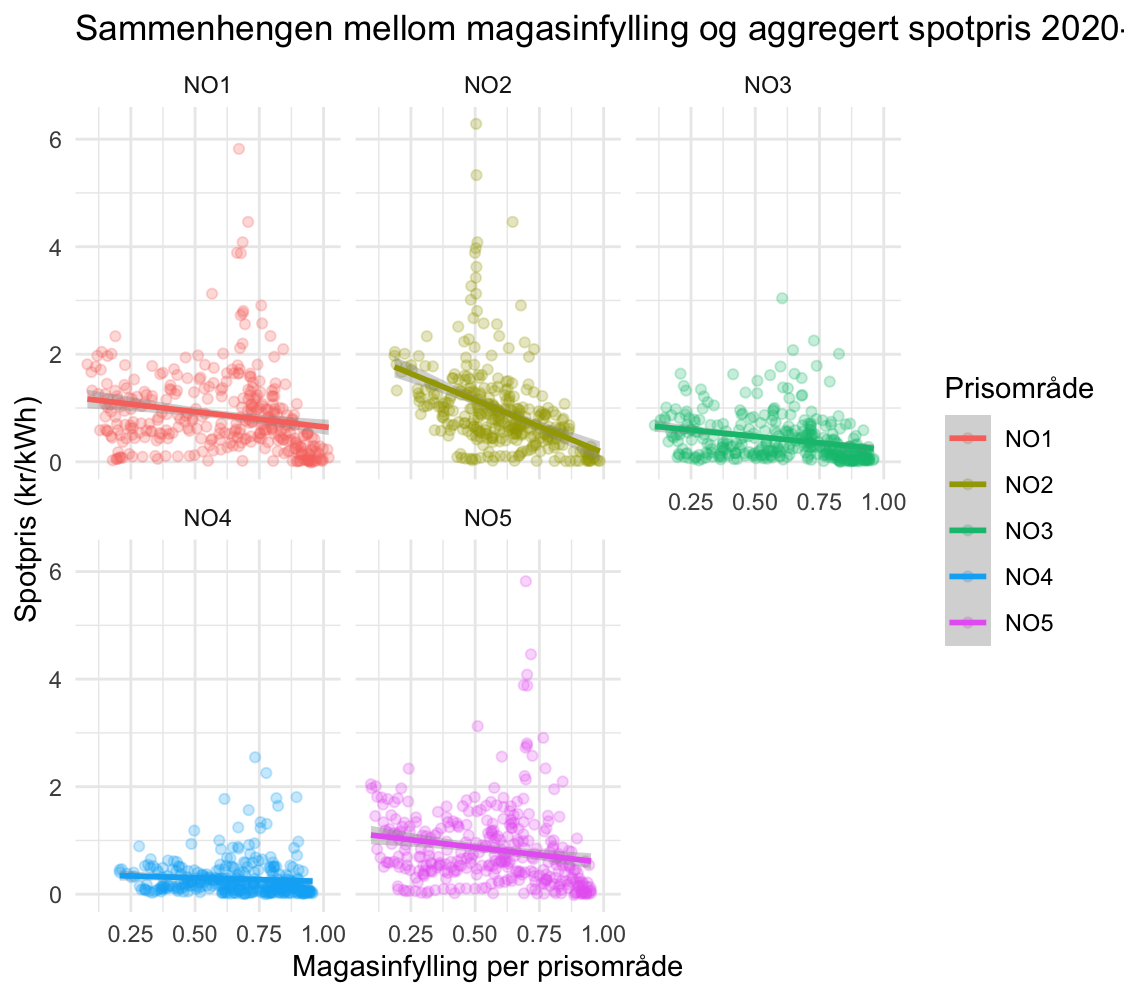
\includegraphics[width=3.25in,height=\textheight,keepaspectratio]{Problemstilling 3/Magfyll_spott_peromrade_2020_26.png}

}

\caption{Figur 4.4: Magainsinfylling og spotpris}

\end{figure}%

Figur 4.4 gir en første indikasjon på hvordan spotprisene varierer med
magasinfyllingen, og om sammenhengen ser ut til å være forskjellig
mellom prisområdene. For å undersøke denne sammenhengen nærmere, og
samtidig ta hensyn til geografiske forskjeller og utviklingen over tid,
estimeres det deretter en OLS-regresjonsmodell.

\paragraph{4.4.3 OLS-regresjon}\label{ols-regresjon}

For å undersøke sammenhengen mellom magasinfylling og spotpris,
kontrollert for geografiske forskjeller og tidstrender, estimeres en
OLS-regresjonsmodell. Prisområde inkluderes som kategorisk variabel,
mens dato inngår som en lineær tidstrend.

\begin{longtable}[]{@{}lrrll@{}}
\caption{OLS-regresjon: Magasinfylling og spotpriser}\tabularnewline
\toprule\noalign{}
Variabel & Koeffisient & Standardfeil & p-verdi & Signifikans \\
\midrule\noalign{}
\endfirsthead
\toprule\noalign{}
Variabel & Koeffisient & Standardfeil & p-verdi & Signifikans \\
\midrule\noalign{}
\endhead
\bottomrule\noalign{}
\endlastfoot
Magasinfylling & -0.6716 & 0.0666 & \textless0.001 & *** \\
Dato & 0.0001 & 0.0000 & \textless0.001 & *** \\
\end{longtable}

\emph{Merknad: NO1 er referanseområdet. Standardfeil rapporteres sammen
med koeffisientene.} \textbf{,} og * angir statistisk signifikans på
henholdsvis 0,1-, 1- og 5-prosentnivå.*

Modellen er estimert med 1 760 observasjoner og har en R² på 0,213 og en
justert R² på 0,211. Dette innebærer at modellen forklarer omtrent 21,1
prosent av variasjonen i spotprisene, justert for antall
forklaringsvariabler.

Koeffisienten for magasinfylling er −0,6716 og statistisk signifikant på
0,1-prosentnivå. Ettersom fyllingsgraden er målt fra 0 til 1, innebærer
dette at en økning i fyllingsgraden på 10 prosentpoeng er forbundet med
en reduksjon i spotprisen på omtrent 0,067 kr/kWh, kontrollert for
prisområde og dato. Resultatet indikerer dermed en negativ sammenheng
mellom magasinfylling og spotpris.

Regresjonen viser også geografiske forskjeller i spotprisene. NO3 og NO4
har henholdsvis 0,451 og 0,547 kr/kWh lavere spotpriser enn NO1,
kontrollert for magasinfylling og dato. Begge forskjellene er statistisk
signifikante på 0,1-prosentnivå. For NO2 og NO5 er det ikke statistisk
signifikante forskjeller sammenlignet med NO1.

Datovariabelen har en positiv koeffisient på 0,0001423 og er statistisk
signifikant på 0,1-prosentnivå. Dette indikerer en positiv lineær
tidstrend i spotprisene gjennom analyseperioden. Koeffisienten tilsvarer
en økning på omtrent 0,000142 kr/kWh per dag, eller 0,052 kr/kWh per år.

\subsection{5. Konklusjon}\label{konklusjon}

Oppgaven har undersøkt sammenhenger mellom Norgespris, strømpriser,
husholdningenes strømforbruk og magasinfylling i Norge. Analysen av
husholdningenes strømforbruk viser at OLS- og LASSO-modellene har
tilnærmet lik prediksjonsevne. Dette tyder på at LASSO ikke gir noen
vesentlig forbedring sammenlignet med OLS i denne analysen.

\textbf{For problemstilling 2 viser analysen a}t. \textbf{\textless-
Bendik}

Videre finner analysen en negativ og statistisk signifikant sammenheng
mellom magasinfylling og spotpriser. Høyere magasinfylling er dermed
forbundet med lavere spotpriser, også når det kontrolleres for
prisområde og tidsutvikling.

\textbf{Samlet viser analysene at strømforbruk, adopsjon av Norgespris
og spotpriser henger sammen med ulike forhold ved strømmarkedet.
Resultatene må imidlertid tolkes som statistiske sammenhenger, og ikke
nødvendigvis som uttrykk for årsakssammenhenger. \textless- Bendik}

\subsection{6. Bruk av KI}\label{bruk-av-ki}

KI har blitt brukt på litt ulike måter. For enkelhetsskyld starter vi
med å nevne hvilke KI platformer som har blitt brukt: GPTUiO, ChatGPT,
\textbf{Bendik} Gemini.

Opplever at ChatGPT er bedre til å assistere med feilsøking i koden,
idemyldring og språk, mens GPT UiO er bedre for håndtere større mengder
data for å se sammenhenger da den har større minne enn ChatGPT. Med
større mengder data menes lengre koder, og større feilsøkingsprossessert
der minnet til ChatGPT ofte går tomt og man ønsker å beholde
kontinuiteten i feilsøkingen i stede for å opprette nytt samtalevindu
hver gang minnet for den samtaletråden er full. Begge modellene har
assistert med å rense koder, forbedre koder og feilsøke. Forklaringer på
hvordan vi har arbeidet med KI kommer under. Enkelte korte formuleringer
og standardiserte kodeuttrykk er være beholdt uendret når det er
begrenset rom for meningsfull alternativ formulering, for eksempel ved
enkle faktabeskrivelser eller vanlig R-syntaks. Dette gjelder ikke
faglige vurderinger, analyser eller tolkninger, som er utarbeidet av
oss.

\subsubsection{6.1 KI og idemyldring for
problemstillinger}\label{ki-og-idemyldring-for-problemstillinger}

KI er brukt til å komme med forslag til formulering til
problermsstillinger basert på vår temmatiske ide og ønsker om vinkling.
Disse forslagene har blitt bearbeidet videre av oss, både i form av at
vi har kombinert flere av formuleringene da vi opplever at forslagene
kommer til kort, men også underveis i arbeidsprosessen når vi har bedre
oversikt over dataen vi har samlet.

\subsubsection{6.2. KI, koding og
feilsøking}\label{ki-koding-og-feilsuxf8king}

KI er brukt for å hjelpe med å generere koder. Hvis man ikke har funnet
svar på problemer eller spørsmål i online forum som f.eks. Stackoverflow
er KI brukt til å spørre om hvilke pakker eller metode man kan bruke for
å feks. endre datasettet i NVE på fyllingsgrad slik at det ikke bare
sorteres på uke, men også dag. Det var nødvendig for å kunne sette det
sammen til et stort historisk sett og unngå å få flere NA verdier. KI
ble brukt til å foreslå og forklare standard R-syntaks for innlesing og
bearbeiding av data. Vi tok selv stilling til hvilke filer som skulle
inngå, hvordan filene var strukturert, hvilke rader som skulle hoppes
over, og hvordan resultatet skulle valideres og brukes videre i
analysen. Et eksempel er innlesing av flere Excel-filer ved hjelp av
lapply() og read\_excel(). KI kunne foreslå standard syntaks for dette,
mens vi vurderte filutvalget, at de fire første radene skulle hoppes
over, og kontrollerte at dataene ble lest inn riktig.

Et annet konkret eksempel er hvordan KI ble brukt for å endre en gammel
kode for å pivote flere rådatasett om strømmåler og Norgespris (rådataen
fra elhub, gammel kode finnes i mappen gamle scrips og heter maaler.R).
Dette var en tung kode som la sammen et stort datasett, og koden ble
repetert flere ganger. KI ble gitt denne koden og bedt om å gjøre det om
til en funksjon for å gjøre koden kortre og mer leselig. Dog, en
funksjon vil ofte bruke lengre tid på å kjøre enn en manuel pivoting,
men kan man bruke én funksjon på flere datasett som har samme struktur i
stede for å repitere samme kode flere ganger. Ved å få KI til å endre
det til en funksjon gikk vi fra 87 linjer med effektiv kode til 48
linjer. Dersom man ønsker å gjennta samme undersøkelser senere når det
kommer mer data for Norgespris og strømmåler kan man dermed bare bruke
en funksjon og ikke måtte kode alt manuelt.

KI er brukt som et supplement til online forum for å hjelpe med å forstå
feilkoder fra RStudio, og feilkoder fra Quatro. Spesieltt i Quarto er KI
brukt for å forstå feilkodene, og til å backtracke arbeid. Feilen har
ofte skyldtes at man har glemt å kopiere inn alle endringene som er
gjort i koden(e) i RStudio scripts over til Quarto slik at den kjører på
feil verdier eller variabler som er endret. Det samme problemet har
skjedd i RStudio. Vi har flere scripts og noen av de bygger på/krever
resultate for andre. Har man gjort en endring i ett og glemt å
videreføre det oppstår det problemer.

\subsubsection{6.3. KI og skriving}\label{ki-og-skriving}

KI ble brukt til å foreslå struktur og tekstutkast til deler av
oppgaven. Verktøyet fikk som utgangspunkt materiale utarbeidet av oss
selv, herunder introduksjon, problemstillinger, kode, beskrivelser av
databehandling og metode i punktform. KI ble deretter bedt om å foreslå
en kapittelstruktur og omarbeide punktvise beskrivelser til
sammenhengende tekst. Materialet inkluderte også relevante deler av
pensum og faglige kilder som gruppen hadde identifisert gjennom lesing,
forelesninger og egne notater. KI ble ikke brukt som faglig kilde. Alle
tekstforslag fra KI ble gjennomgått, kontrollert og bearbeidet av oss.
Vi kontrollerte særlig at beskrivelsene var i samsvar med det faktiske
arbeidet som var gjennomført, og at faglige påstander og
kildehenvisninger var korrekte og basert på originalkildene. Vi er
ansvarlig for den endelige teksten, analysen og de faglige vurderingene.
KI ble også brukt til språkvask, inkludert kontroll av skrivefeil og
forslag til oppstamming av teskt.

\subsection{7. Kilder}\label{kilder}

\phantomsection\label{refs}
\begin{CSLReferences}{1}{0}
\bibitem[\citeproctext]{ref-athey_machine_2019}
Athey, Susan, and Guido W. Imbens. 2019. {``Machine Learning Methods
That Economists Should Know About.''} \emph{Annual Review of Economics}
11: 685--725.
\url{https://doi.org/10.1146/annurev-economics-080217-053433}.

\bibitem[\citeproctext]{ref-energidepartementet_norgespris_2025}
Energidepartementet. 2025. {``Norgespris På Strøm Og Fjernvarme.''}
Offentlige myndigheter. \emph{Regjeringen}.
\url{https://www.regjeringen.no/no/tema/energi/strom/norgespris-pa-strom-og-fjernvarme/id3120995/}.

\bibitem[\citeproctext]{ref-energidepartementet_norgespris_2026}
---------. 2026. {``Norgespris for 2027 Kan Bestilles Fra 5. Januar.''}
Offentlige myndigheter. \emph{Regjeringen}.
\url{https://www.regjeringen.no/no/aktuelt/norgespris-for-2027-kan-bestilles-fra-5.-januar/id3186516/}.

\bibitem[\citeproctext]{ref-norges_vassdrag_og_energidirektorat_magasinstatistikk_2026}
energidirektorat, Norges vassdrag og. 2026. {``Magasinstatistikk
(\%).''}
\url{https://www.nve.no/energi/analyser-og-statistikk/magasinstatistikk/}.

\bibitem[\citeproctext]{ref-fonti_feature_2017}
Fonti, Valeria. 2017. {``Feature Selection Using LASSO.''} VU Amsterdam.
\url{https://vu-business-analytics.github.io/internship-office/papers/paper-fonti.pdf}.

\bibitem[\citeproctext]{ref-gentzkow_text_2019}
Gentzkow, Matthew, Bryan Kelly, and Matt Taddy. 2019. {``Text as
Data.''} \emph{Journal of Economic Literature} 57 (3): 535--74.
\url{https://doi.org/10.1257/jel.20181300}.

\bibitem[\citeproctext]{ref-hammersmark_econ3170_2026}
Hammersmark, Eirik Brandsaas. 2026. {``ECON3170: Data Science for
Økonomer.''} Forelesningsnotater og kursmateriell, Universitetet i Oslo.

\bibitem[\citeproctext]{ref-hastie_elements_2009}
Hastie, Trevor, Robert Tibshirani, and Jerome Friedman. 2009. \emph{The
Elements of Statistical Learning: Data Mining, Inference, and
Prediction}. 2nd ed. Springer.

\bibitem[\citeproctext]{ref-statsministerens_kontor_regjeringen_2021}
kontor, Statsministerens, Energidepartementet, and Finansdepartementet.
2021. {``Regjeringen Med Milliardpakke i Strømstøtte.''} Offentlige
myndigheter. \emph{Regjeringen}.
\url{https://www.regjeringen.no/no/aktuelt/regjeringen-med-milliardpakke-i-stromstotte/id2891839/}.

\bibitem[\citeproctext]{ref-kuhn_tidy_2023}
Kuhn, Max, and Julia Silge. 2023. \emph{Tidy Modeling with r}. Version
1.0.0. O'Reilly. \url{https://www.tmwr.org/}.

\bibitem[\citeproctext]{ref-nordpool_price_2026}
Nordpool. 2026a. {``Price Indices.''}
\href{https://Price\%20indices}{Price indices}.

\bibitem[\citeproctext]{ref-nordpool_prices_2026}
---------. 2026b. {``Prices.''}
\url{https://data.nordpoolgroup.com/auction/day-ahead/prices?deliveryDate=latest&currency=NOK&aggregation=DailyAggregate&deliveryAreas=AT,NO1,NO2,NO3,NO4,NO5}.

\bibitem[\citeproctext]{ref-sannes_norgespris_2026-1}
Sannes, Christoffer, and Elhub. 2026a. {``Norgespris Antall Per Kommune,
Forbruksgruppe Og Dag.''}
\url{https://elhub.no/data-og-innsikt/datakatalog}.

\bibitem[\citeproctext]{ref-sannes_norgespris_2026}
---------. 2026b. {``Norgespris Antall Per Prisområde, Forbruksgruppe Og
Dag.''} Telling for antall målepunkt med \{Norgespriskontrakt\} per
prisområde og dag. \{Tellingen\} er gjort for forbruksgruppene
husholdningog fritidsboligslik at man kan følge dem separat.
\url{https://elhub.no/data-og-innsikt/datakatalog}.

\bibitem[\citeproctext]{ref-skaansar_kraftaret_2022}
Skaansar, Ellen. 2022. {``Kraftåret 2021 - Historisk Høye
Kraftpriser,''} August.
\url{https://www.nve.no/nytt-fra-nve/nyheter-energi/kraftaret-2021-historisk-hoye-kraftpriser/}.

\bibitem[\citeproctext]{ref-stokke_hammer-dybvad_forbruk_2026}
Stokke Hammer-Dybvad, Alexander, and Elhub. 2026. {``Forbruk Per
{Norgespris}-Status, Forbruksgruppe, Prisområde Og Antall Målepunker Per
Time.''} \url{https://elhub.no/data-og-innsikt/datakatalog}.

\bibitem[\citeproctext]{ref-tibshirani_regression_1996}
Tibshirani, Robert. 1996. {``Regression Shrinkage and Selection via the
Lasso.''} \emph{Journal of the Royal Statistical Society: Series B
(Methodological)} 58 (1): 267--88.
\url{https://doi.org/10.1111/j.2517-6161.1996.tb02080.x}.

\bibitem[\citeproctext]{ref-wickham_r_2016}
Wickham, Hadley, and Garrett Grolemund. 2016. \emph{R for Data Science:
Import, Tidy, Transform, Visualize, and Model Data}. First edition.
Sebastopol, CA: O'Reilly.

\end{CSLReferences}

\subsection{8. Vedlegg}\label{vedlegg}

\begin{Shaded}
\begin{Highlighting}[]
\CommentTok{\#kan legge til alt vi vil ha med som vedlegg i bloks her. Må ta stilling til om vi skal legge alle kodene som er brukt (altså de som kjører i bakgrunnen her + evt noen flere) her eller om de bare skal være del av zip{-}filen. Jeg tenker vi bare kan legge alt her, i samme rekkefølge som det diskluteres og nevnes i oppgaven. }
\end{Highlighting}
\end{Shaded}





\end{document}
